%%----------------------------------------------------------------------------
%% Presentatie HoGent Bedrijf en Organisatie
%%----------------------------------------------------------------------------
%% Auteur: Bert Van Vreckem [bert.vanvreckem@hogent.be]

\documentclass{beamer}

%==============================================================================
% Aanloop
%==============================================================================

%---------- Packages ----------------------------------------------------------

\usepackage{graphicx,multicol}
\usepackage{comment,enumerate,hyperref}
\usepackage{amsmath,amsfonts,amssymb}
\usepackage{tikz}
\usepackage[dutch]{babel}
\usepackage[utf8]{inputenc}
\usepackage{multirow}
\usepackage{eurosym}
\usepackage{listings}
\usepackage[T1]{fontenc}
\usepackage{lmodern}
\usepackage{textcomp}
\usepackage{framed}
\usepackage{wrapfig}
\usepackage{pgf-pie}
\usepackage{pgfplots}

%---------- Configuratie ------------------------------------------------------

\usetikzlibrary{arrows,shapes,backgrounds,positioning,shadows}
\usetikzlibrary{pgfplots.statistics}

\usetheme{hogent}

%---------- Commando-definities -----------------------------------------------

\newcommand{\tabitem}{~~\llap{\textbullet}~~}

%---------- Info over de presentatie ------------------------------------------

\title[Intro]{Onderzoekstechnieken\\Les 2. Analyse op 1 variabele}
\author{Anita Bernard, Jens Buysse, Bert {Van Vreckem}}

\date{AY 2016-2017}


%==============================================================================
% Inhoud presentatie
%==============================================================================

\begin{document}

%---------- Front matter ------------------------------------------------------

% Dia met het HoGent logo
\HoGentLogo

% Titeldia met faculteitslogo
\titleframe

%---------- Inhoud ------------------------------------------------------------

\begin{frame}
  \frametitle{What's on the menu today?}

  \tableofcontents
\end{frame}

\begin{frame}
  \frametitle{Stel, je wil een vriendengroep analyseren}

  Vragen die je kan stellen:

  \begin{itemize}
    \item Wat is de grootte van mijn vrienden?
    \item Hoeveel wegen mijn vrienden?
    \item Hoe veilig maken ze hun woonomgeving?
    \item Hebben ze familie?
    \item \ldots
  \end{itemize}
\end{frame}

\begin{frame}
  \frametitle{Hoe groot zijn mijn vrienden?}

  \begin{tikzpicture}[xscale=4,yscale=2]
      \draw (0,2) -- (0,0);
      \foreach \num/\label in {0/0, 0.2/20, .4/40, .6/60, .8/80, 1/100, 1.2/120, 1.4/140, 1.6/160, 1.8/180, 2/200}{%
        \draw (0, \num) -- (2.5, \num);
        \draw[shift={(0, \num)}] (1pt,0pt) -- (-1pt,0pt) node[left] {\scriptsize \label};
      }

      \node[anchor=north] (hero1) at (0.3,1.5)
        {\includegraphics[height=2.9cm]{img/les2-hero-1}};
      \node[anchor=north] (hero2) at (0.8,2.05)
        {\includegraphics[height=4cm]{img/les2-hero-2}};
      \node[anchor=north] (hero3) at (1.3,1.575)
        {\includegraphics[height=3.1cm]{img/les2-hero-3}};
      \node[anchor=north] (hero4) at (1.8,2.1)
        {\includegraphics[height=4.1cm]{img/les2-hero-4}};
      \node[anchor=north] (hero5) at (2.3,1.95)
        {\includegraphics[height=3.8cm]{img/les2-hero-5}};

        \node (size1) at (0.3, 1.5) {\scriptsize 141 cm};
        \node (size2) at (0.8, 2.1) {\scriptsize 198 cm};
        \node (size3) at (1.3, 1.51) {\scriptsize 143 cm};
        \node (size4) at (1.8, 2.15) {\scriptsize 201 cm};
        \node (size5) at (2.3, 1.95) {\scriptsize 184 cm};
    \end{tikzpicture}
\end{frame}

\section{Beschrijvende statistiek}

\subsection{Centrummaten}

\sectionframelogo{Centrummaten}

\begin{frame}
  \frametitle{Gemiddelde (of \emph{mean}, \emph{average})}

  \brightbox{Het \textcolor{HoGentAccent6}{gemiddelde} is de som van alle waarden gedeeld door het aantal waarden}

    \begin{columns}[c]
    \column{.4\textwidth}
    \begin{center}
      \begin{tabular}{|c|c|c|c|c|}
        \hline
        $x_1$ & $x_2$ & $x_3$ & $x_4$ & $x_5$ \\
        \hline
        141 & 198 & 143 & 201 & 184 \\
        \hline
      \end{tabular}
    \end{center}
    \column{.4\textwidth}
    \begin{center}
      \includegraphics[width=.6cm]{les2-hero-1}
      \includegraphics[width=.6cm]{les2-hero-2}
      \includegraphics[width=.6cm]{les2-hero-3}
      \includegraphics[width=.6cm]{les2-hero-4}
      \includegraphics[width=.6cm]{les2-hero-5}
    \end{center}
  \end{columns}


  \vspace{.5cm}
  \begin{description}
    \item[Vraag 1] Het gemiddelde van 15 cijfers is 12. Welk nummer moeten we aan de rij van cijfers toevoegen om een gemiddelde van 13 te komen?
    \item[Vraag2] Wat gebeurt er als Kabouter Wesley (10cm) er bij komt?
  \end{description}

  \hfill \includegraphics[width=4cm]{img/les2-hero-6}

\end{frame}

\begin{frame}
  \frametitle{Mediaan (\emph{median})}

  \brightbox{Om de \textcolor{HoGentAccent6}{mediaan} te vinden, sorteer de waarden en kies het middelste nummer}

  \begin{itemize}
    \item Oneven aantal getallen: geen probleem
    \item Even aantal getallen: gemiddelde van de middelste twee
  \end{itemize}

    \begin{columns}[c]
    \column{.4\textwidth}
    \begin{center}
      \begin{tabular}{|c|c|c|c|c|}
        \hline
        $x_1$ & $x_2$ & $x_3$ & $x_4$ & $x_5$ \\
        \hline
        141 & 198 & 143 & 201 & 184 \\
        \hline
      \end{tabular}
    \end{center}
    \column{.4\textwidth}
    \begin{center}
      \includegraphics[width=.6cm]{les2-hero-1}
      \includegraphics[width=.6cm]{les2-hero-2}
      \includegraphics[width=.6cm]{les2-hero-3}
      \includegraphics[width=.6cm]{les2-hero-4}
      \includegraphics[width=.6cm]{les2-hero-5}
    \end{center}
  \end{columns}


  \pause

  \begin{description}
    \item[Vraag 1] Wat gebeurt er nu als Kabouter Wesley er bij komt?
    \item[Vraag 2] Gegeven het totaal aantal mensen gered door Batman de laatste 8 jaar, wat is de mediaan?
  \end{description}

    \centering
    \begin{tabular}{|c|c|c|c|c|c|c|c|}
      \hline
      4 & 7 & 11 & 16 & 20 & 22 & 25 & 26 \\
      \hline
    \end{tabular}
    \includegraphics[width=.6cm]{img/les2-hero-2}
\end{frame}

\begin{frame}
  \frametitle{Modus (\emph{mode})}

  \brightbox{De \textcolor{HoGentAccent6}{modus} is het vaakst voorkomende getal in een reeks getallen}

  Totaal aantal mensen gered door Superman de laatste 15 jaar:

   \begin{center}
    \begin{tabular}{|c|c|c|c|c|c|c|c|c|c|c|c|c|c|c|}
      \hline
      3&7&5&13&20&23&39&23&40&23&14&12&56&23&29\\
      \hline
    \end{tabular}
    \includegraphics[width=.7cm]{img/les2-hero-3}
  \end{center}


  Totaal aantal mensen gered door Batman de laatste 8 jaar:
  \begin{center}
    \begin{tabular}{|c|c|c|c|c|c|c|c|}
      \hline
      4 & 7 & 11 & 16 & 20 & 22 & 25 & 26 \\
      \hline
    \end{tabular}

    \includegraphics[width=.6cm]{img/les2-hero-2}
  \end{center}

\end{frame}

\subsection{Spreidingsmaten}
\sectionframelogo{Spreidingsmaten}

\begin{frame}
  \frametitle{Bereik (\emph{range})}

  \brightbox{Het \textcolor{HoGentAccent6}{bereik} van een reeks getallen is de absolute waarde van het verschil tussen het grootste en kleinste getal in de reeks.}

    \begin{columns}[c]
    \column{.4\textwidth}
    \begin{center}
      \begin{tabular}{|c|c|c|c|c|}
        \hline
        $x_1$ & $x_2$ & $x_3$ & $x_4$ & $x_5$ \\
        \hline
        141 & 198 & 143 & 201 & 184 \\
        \hline
      \end{tabular}
    \end{center}
    \column{.4\textwidth}
    \begin{center}
      \includegraphics[width=.6cm]{les2-hero-1}
      \includegraphics[width=.6cm]{les2-hero-2}
      \includegraphics[width=.6cm]{les2-hero-3}
      \includegraphics[width=.6cm]{les2-hero-4}
      \includegraphics[width=.6cm]{les2-hero-5}
    \end{center}
  \end{columns}


\end{frame}

\begin{frame}
  \frametitle{Kwartielen (\emph{quartiles})}

  \brightbox{De \textcolor{HoGentAccent6}{kwartielen} van een gesorteerde reeks getallen zijn de waarden die de lijst in vier gelijke delen verdeelt. Elk deel vormt dus een kwart van de dataset. Men spreekt van een eerste, tweede en derde kwartiel, genoteerd als resp,~$Q_1$, $Q_2$, $Q_3$}

  \vspace{1cm}

  Totaal aantal mensen gered door Superman de laatste 15 jaar:
   \begin{center}
    \begin{tabular}{|c|c|c|c|c|c|c|c|c|c|c|c|c|c|c|}
      \hline
      3&7&5&13&20&23&39&23&40&23&14&12&56&23&29\\
      \hline
    \end{tabular}
    \includegraphics[width=.7cm]{img/les2-hero-3}
  \end{center}

\end{frame}

\begin{frame}
  \frametitle{Variantie (\emph{variance}) en standaardafwijking (\emph{standard deviation})}

  \brightbox{De \textcolor{HoGentAccent6}{variantie} is het gemiddelde gekwadrateerde verschil tussen de elementen van de dataset en zijn gemiddelde}

  \vspace{1em}
  \brightbox{De \textcolor{HoGentAccent6}{standaardafwijking} is de vierkantswortel van de variantie}

    \begin{columns}[c]
    \column{.4\textwidth}
    \begin{center}
      \begin{tabular}{|c|c|c|c|c|}
        \hline
        $x_1$ & $x_2$ & $x_3$ & $x_4$ & $x_5$ \\
        \hline
        141 & 198 & 143 & 201 & 184 \\
        \hline
      \end{tabular}
    \end{center}
    \column{.4\textwidth}
    \begin{center}
      \includegraphics[width=.6cm]{les2-hero-1}
      \includegraphics[width=.6cm]{les2-hero-2}
      \includegraphics[width=.6cm]{les2-hero-3}
      \includegraphics[width=.6cm]{les2-hero-4}
      \includegraphics[width=.6cm]{les2-hero-5}
    \end{center}
  \end{columns}

\end{frame}

\begin{frame}
  \frametitle{Eigenschappen standaardafwijking}

  \begin{itemize}
    \item<+-> Kan de standaardafwijking negatief zijn?
    \item<+-> Wat is de kleinst mogelijke waarde? Wat duidt dit aan?
    \item<+-> Wat is de invloed van uitschieters op de standaardafwijking?
    \item<+-> In welke eenheden staat de standaarddeviatie?
    \item<+-> Hoe interpreteer je de standaardafwijking in combinatie met het gemiddelde?
  \end{itemize}
\end{frame}

\begin{frame}[plain]

  \scaledimg{img/les2-01}
\end{frame}

\section{Eenvoudige grafieken}
\sectionframelogo{}

\begin{frame}
  \frametitle{Cirkeldiagram (\emph{pie chart})}

  \centering
  \includegraphics[width=.8cm]{img/les2-hero-3}
  Waarom herkent niemand Superman?
  \begin{tikzpicture}[scale=.5]
    \pie[text=legend,color={HoGentAccent1,HoGentAccent2,HoGentAccent3}]{%
    3/Heeft herkend, 5/Twijfelt, 92/Lijdt aan prosopagnosia}
  \end{tikzpicture}

\end{frame}

\begin{frame}
  \frametitle{Cirkeldiagram}

  Voordelen:
  \begin{itemize}
    \item Met percentages rond 20\% kan je makkelijk verduidelijken t.o.v. volledige dataset
  \end{itemize}
  Nadelen:
  \begin{itemize}
    \item Vergelijken op basis van hoek, terwijl lengte intuïtiever is
    \item Figuur onduidelijk bij veel categorieën
  \end{itemize}

  \begin{center}
  \brightbox{Gebruik een cirkeldiagram zo weinig mogelijk!}
  \includegraphics[width=.6\textwidth]{img/pie-chart.png}
  \end{center}

\end{frame}

\begin{frame}
  \frametitle{Staafdiagram (\emph{bar chart})}

  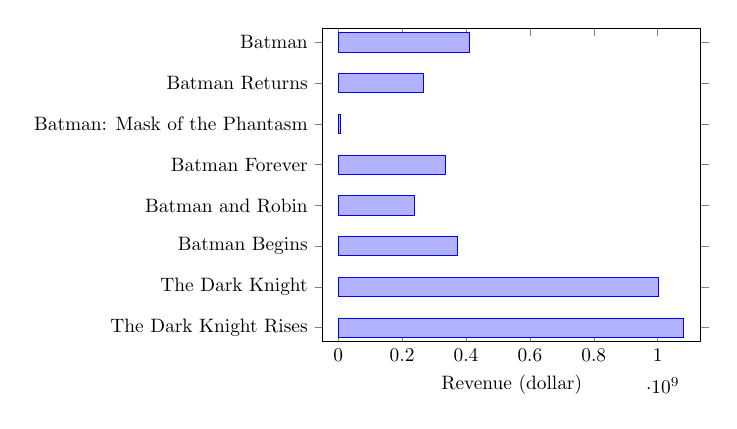
\begin{tikzpicture}[scale=.7]
    \begin{axis}[
      xbar,
      enlargelimits=0.05,
      legend style={at={(0.5,-0.2)}, anchor=north,legend columns=-1},
      ytick=data,
      symbolic y coords={The Dark Knight Rises, The Dark Knight, Batman Begins, Batman and Robin, Batman Forever, Batman: Mask of the Phantasm, Batman Returns, Batman},
      xlabel=Revenue (dollar)
    ]
    \addplot
    coordinates {
      (1080472000,The Dark Knight Rises)
      (1002000000,The Dark Knight)
      (372710000,Batman Begins)
      (238207000,Batman and Robin)
      (336529000,Batman Forever)
      (5617000,Batman: Mask of the Phantasm)
      (266822000,Batman Returns)
      (411348000,Batman)};
  \end{axis}
\end{tikzpicture}
\end{frame}

\begin{frame}
  \frametitle{Staafdiagram}
  % Source: http://mirrors.ibiblio.org/CTAN/graphics/pgf/contrib/pgfplots/doc/pgfplots.pdf
  % p.79
  \begin{center}
    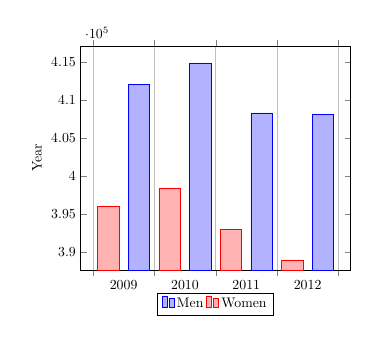
\begin{tikzpicture}[scale=.5]
      \begin{axis}[
          x tick label style={
          /pgf/number format/1000 sep=},
          ylabel=Year,
          enlargelimits=0.05,
          legend style={at={(0.5,-0.1)},
        anchor=north,legend columns=-1},
        ybar interval=0.7,
      ]
      \addplot
      coordinates {(2012,408184) (2011,408348)
      (2010,414870) (2009,412156) (2008,415 838)};
      \addplot
      coordinates {(2012,388950) (2011,393007)
      (2010,398449) (2009,395972) (2008,398866)};
      \legend{Men,Women}
    \end{axis}
  \end{tikzpicture}
\end{center}
Voordelen:

\begin{itemize}
  \item Makkelijker vergelijken van categorieën
  \item Per categorie meerdere ``bars'' mogelijk
\end{itemize}
\end{frame}


\begin{frame}
  \frametitle{Boxplot}

  % Source: http://mirrors.ibiblio.org/CTAN/graphics/pgf/contrib/pgfplots/doc/pgfplots.pdf
  % p.430
  \begin{tikzpicture}
    \begin{axis}[x=3cm,xticklabels={},xmax=2.3]
      \addplot+[
        boxplot prepared={
          draw direction=y,
          lower whisker=5,
          lower quartile=7,
          median=8.5,
          upper quartile=9.5,
          upper whisker=10,
        },
      ]
      table[row sep=\\,y index=0] {
        data\\ 1\\ 3\\
      }
      [right,color=HoGentAccent2]
      node at
      (boxplot box cs: 1,.6)
      {uitschieter}
      node at
      (boxplot box cs: \boxplotvalue{lower quartile},1)
      {$Q_3$}
      node at
      (boxplot box cs: \boxplotvalue{median},1)
      {$Q_2$, mediaan}
      node at
      (boxplot box cs: \boxplotvalue{upper quartile},1)
      {$Q_1$}
      node at
      (boxplot box cs: \boxplotvalue{upper whisker},1)
      {max}
      ;
    \end{axis}
  \end{tikzpicture}

  Voordeel: snelle manier om data te inspecteren en verschillende datasets te vergelijken
\end{frame}

\section{Interpretatie van grafieken}
\sectionframelogo{Valkuilen}

\begin{frame}
  \frametitle{Data-ambiguïteit}

  = Vergeten aan te duiden wat de data betekent.
  \vspace{1cm}

  \begin{columns}
    \column{.5\textwidth}
    \includegraphics[width=\textwidth]{img/les2-02}
    \column{.5\textwidth}
    Tips:
    \begin{itemize}
      \item Benoem je assen
      \item Geef een duidelijke titel
      \item Benoem de meeteenheid (en evt. grootorde)
      \item Voeg een bijschrift toe met uitleg over de grafiek
    \end{itemize}
  \end{columns}
\end{frame}

\begin{frame}
  \frametitle{Data distortion}

  = Verkeerde conclusies laten trekken uit een grafische voorstelling

  \begin{center}
    \includegraphics[width=.7\textwidth]{img/les2-03}
  \end{center}
\end{frame}

\begin{frame}
  \frametitle{Data distortion}

  \begin{center}
    \includegraphics[width=.8\textwidth]{img/les2-03-2}
  \end{center}
\end{frame}

\begin{frame}
  \frametitle{Data distraction}

  \begin{itemize}
    \item Vermijd toeters en bellen in je grafieken
    \item Minimaliseer inkt tot data ratio
  \end{itemize}

  \centering
  \includegraphics[width=.4\textwidth]{img/les2-04}
  \includegraphics[width=.4\textwidth]{img/les2-05}

  \includegraphics[width=.4\textwidth]{img/les2-06}
  \includegraphics[width=.4\textwidth]{img/les2-07}
\end{frame}

\begin{frame}
  \frametitle{Anscombe's Quartet}

  \centering
  \includegraphics[width=.8\textwidth]{img/anscombes_quartet}

  Vier verschillende datasets met dezelfde statistische eigenschappen. Deze tonen het belang aan van data-visualisatie.
\end{frame}

\end{document}
